%% LyX 2.4.4 created this file.  For more info, see https://www.lyx.org/.
%% Do not edit unless you really know what you are doing.
\documentclass[english]{article}
\usepackage[T1]{fontenc}
\usepackage[latin9]{inputenc}
\usepackage{units}
\usepackage{enumitem}
\usepackage{amsmath}
\usepackage{amsthm}
\usepackage{cancel}
\usepackage{geometry}
\geometry{verbose,tmargin=1in,bmargin=1in,lmargin=1in,rmargin=1in}
\PassOptionsToPackage{normalem}{ulem}
\usepackage{ulem}

\makeatletter
%%%%%%%%%%%%%%%%%%%%%%%%%%%%%% Textclass specific LaTeX commands.
\numberwithin{equation}{section}
\numberwithin{figure}{section}
\newlength{\lyxlabelwidth}      % auxiliary length 

%%%%%%%%%%%%%%%%%%%%%%%%%%%%%% User specified LaTeX commands.
\usepackage{fancyhdr}
\usepackage{lastpage}
\pagestyle{fancy}
\usepackage{enumitem}
\usepackage{ifthen}
%sets math fonts to be more readable
\everymath=\expandafter{\the\everymath\displaystyle}
%\DeclareMathSizes{10}{10}{10}{10}
\usepackage{multicol}

\usepackage{tikz}
\usetikzlibrary{plotmarks}
\usepackage{pgfplots}
\pgfplotsset{compat=newest}

\usepackage{calc}
\usepackage[nomessages]{fp}

\usepackage{advdate}    % Advancing/saving dates
\usepackage{datetime}   % Dates formatting
\usepackage{datenumber} % Counters for dates
% Added by lyx2lyx
\setlength{\parskip}{\smallskipamount}
\setlength{\parindent}{0pt}

\makeatother

\usepackage{babel}
\begin{document}
\renewcommand{\author}{Dr.\,James Ashe}

\newcommand{\classNum}{107}

\newcommand{\classSec}{7 and 10}

\newcommand{\nameType}{}

\newcommand{\examType}{Exam 1 Review Solutions: sections 2.1-2.4}

\renewcommand{\date}{\hfill Exam 1 is on \formatdate{8}{9}{2014}}

%%First page's header%%%%%%%%%%%%%%%%%%%%%%
\fancypagestyle{firststyle} %%header settings for first pagr
{
	\fancyhead[L]{MTH \classNum{}(\classSec{}) \author{}\\
	\textbf{\examType{}} \date{}}
	\fancyhead[C]{\textbf{\nameType}}
	\setlength{\headsep}{14pt}
}
%%%%%%%%%%%%%%%%%%%%%%%%%%%%%%%%%%%%%%%%%%

%%Next page's header%%%%%%%%%%%%%%%%%%%%%%%
%\setlist{nolistsep}
\lhead{MTH \classNum{}(\classSec{})} 
\chead{\textbf{\nameType}} 
\cfoot{\thepage{}~of~\pageref{LastPage}} 
\setlength{\headsep}{5pt} 
%%%%%%%%%%%%%%%%%%%%%%%%%%%%%%%%%%%%%%%%%%%

%%Various settings; see the preamble for other settings%%%%%
%%\setenumerate[0]{leftmargin=12pt,itemindent=0pt,labelwidth=0pt}
\renewcommand{\labelenumi}{\textbf{\arabic{enumi}.}}
\renewcommand{\labelenumii}{\textbf{\alph{enumii}.}}
\thispagestyle{firststyle}
%%%%%%%%%%%%%%%%%%%%%%%%%%%%%%%%%%%%%%%%%%
\newcommand{\xmax}{10}
\newcommand{\xmin}{-10}
\newcommand{\xstep}{0} %must be xmin+n
\newcommand{\ymax}{10}
\newcommand{\ymin}{-10}
\newcommand{\ystep}{0} %must be ymin+n

\newcommand{\xspace}{\vspace{.75cm}}\small
\begin{enumerate}[resume]
\item Let $U=\{1,2,3,4,5,6,7,8\}$ be the universal set, and $A=\{1,2,3,4\}$
and $B=\{4,6,8\}$ be subsets of $U$. Find the indicated set, and
draw a Venn diagram corresponding to the indicated set.\newcommand{\vennScale}{0.5}

\begin{enumerate}
\item $A\cup B$

\begin{enumerate}
\item []$A\cup B=\{1,2,3,4,6,8\}$
\item []%%%%A U B%%%%%
\begin{tikzpicture}[scale=\vennScale]
	\def\circleA{(0,0) circle (1.5)} %A
	\def\circleB{(0:2) circle (1.5)} %B

	\colorlet{circle edgeA}{black!75} 
	\colorlet{circle areaA}{red!50}
	\colorlet{circle edgeB}{black!75} 
	\colorlet{circle areaB}{red!50}

	\tikzset{
		filledA/.style={fill=circle areaA, draw=circle edgeA, thick},
		filledB/.style={fill=circle areaB, draw=circle edgeB, thick},
		outlineA/.style={draw=circle edgeA, thick},
		outlineB/.style={draw=circle edgeB, thick},
	}
	
	\begin{scope}[fill opacity=1.0]         
			\fill[filledB] \circleB;    
			\fill[filledA] \circleA;
	\end{scope}

	\draw[outlineA] \circleA node {$A$}; 
	\draw[outlineB] \circleB node {$B$}; 
	%\node[anchor=south] at (current bounding box.north) {$A \cap B$}; 
	\draw[thick] (-2,-2) rectangle (4,2) node[anchor=south east] at (current bounding box.south east) {$U$}; 
\end{tikzpicture} 
\item []The \emph{Union}:\emph{ }elements\emph{ }in either $A$ \uline{or}
$B$. Note that $A,B\subseteq A\cup B$. Do not repeat elements. \vfill
\end{enumerate}
\item $A\cap B$

\begin{enumerate}
\item []$A\cap B=\{4\}$
\item []%%%%A n B%%%%%
\begin{tikzpicture}[scale=\vennScale]
	\def\circleA{(0,0) circle (1.5)} %A
	\def\circleB{(0:2) circle (1.5)} %B

	\colorlet{circle edgeA}{black!75} 
	\colorlet{circle areaA}{red!50}
	\colorlet{circle edgeB}{black!75} 
	\colorlet{circle areaB}{red!50}

	\tikzset{
		filledA/.style={fill=circle areaA, draw=circle edgeA, thick},
		filledB/.style={fill=circle areaB, draw=circle edgeB, thick},
		outlineA/.style={draw=circle edgeA, thick},
		outlineB/.style={draw=circle edgeB, thick},
	}
	
	\begin{scope}[fill opacity=1.0]    
		\clip \circleA;     
			\fill[filledB] \circleB;
		\clip \circleB;     
			\fill[filledA] \circleA;
	\end{scope}

	\draw[outlineA] \circleA node {$A$}; 
	\draw[outlineB] \circleB node {$B$}; 
	%\node[anchor=south] at (current bounding box.north) {$A \cap B$}; 
	\draw[thick] (-2,-2) rectangle (4,2) node[anchor=south east] at (current bounding box.south east) {$U$}; 
\end{tikzpicture} 
\item []The \emph{intersection}:\emph{ }elements\emph{ }in both $A$ \uline{and}
$B$. Note that $A\cap B\subseteq A,B$. The intersection can be the
empty set, $\emptyset$, e.g., $A\cap A'=\emptyset$.\vfill
\end{enumerate}
\item $A'$

\begin{enumerate}
\item []$A'=\{5,6,7,8\}$
\item []%%%%A'%%%%%
\begin{tikzpicture}[scale=\vennScale]
	\def\circleA{(0,0) circle (1.5)} %A
	\def\circleB{(0:2) circle (1.5)} %B

	\colorlet{circle edgeA}{black!75} 
	\colorlet{circle areaA}{red!100}
	\colorlet{circle edgeB}{black!75} 
	\colorlet{circle areaB}{blue!100}

	\tikzset{
		filledA/.style={fill=circle areaA, draw=circle edgeA, thick},
		filledB/.style={fill=circle areaB, draw=circle edgeB, thick},
		outlineA/.style={draw=circle edgeA, thick},
		outlineB/.style={draw=circle edgeB, thick},
	}

	\draw[thick,fill=red!50,even odd rule] %%even odd rule draws complement of next draw commands%%
		(-2,-2) rectangle (4,2) node[anchor=south east] at (current bounding box.south east) {$U$} 
		\circleA node {$A$};
	\draw[outlineB] \circleB node {$B$}; 
	%\node[below=1pt] at (current bounding box.north) {\footnotesize $A'$}; 

\end{tikzpicture} 
\item []The \emph{complement }of $A$: elements in $U$ but not in $A$.
Note that $A'\cup A=U$. In terms of set difference, 
\begin{eqnarray*}
A' & = & U-A\\
 & = & \{\cancel{1},\cancel{2},\cancel{3},\cancel{4},5,6,7,8\}=\{5,6,7,8\}
\end{eqnarray*}
\vfill.
\end{enumerate}
\item $B'$

\begin{enumerate}
\item []$B'=\{1,2,3,5,7\}$
\item []%%%%B'%%%%%
\begin{tikzpicture}[scale=\vennScale]
	\def\circleA{(0,0) circle (1.5)} %A
	\def\circleB{(0:2) circle (1.5)} %B

	\colorlet{circle edgeA}{black!75} 
	\colorlet{circle areaA}{red!100}
	\colorlet{circle edgeB}{black!75} 
	\colorlet{circle areaB}{blue!100}

	\tikzset{
		filledA/.style={fill=circle areaA, draw=circle edgeA, thick},
		filledB/.style={fill=circle areaB, draw=circle edgeB, thick},
		outlineA/.style={draw=circle edgeA, thick},
		outlineB/.style={draw=circle edgeB, thick},
	}

	\draw[thick,fill=red!50,even odd rule] %%even odd rule draws complement of next draw commands%%
		(-2,-2) rectangle (4,2) node[anchor=south east] at (current bounding box.south east) {$U$} 
		\circleB node {$B$};
	\draw[outlineA] \circleA node {$A$}; 
	%\node[below=1pt] at (current bounding box.north) {\footnotesize $A'$}; 

\end{tikzpicture} 
\begin{eqnarray*}
B' & = & U-B\\
 & = & \{1,2,3,\cancel{4},5,\cancel{6},7,\cancel{8}\}=\{1,2,3,5,7\}
\end{eqnarray*}
\vfill
\end{enumerate}
\item $A\cap B'$

\begin{enumerate}
\item []$A\cap B'=\{1,2,3\}$
\item []%%%%A n B'%%%%%
\begin{tikzpicture}[scale=\vennScale]
	\def\circleA{(0,0) circle (1.5)} %A
	\def\circleB{(0:2) circle (1.5)} %B

	\colorlet{circle edgeA}{black!75} 
	\colorlet{circle areaA}{red!50}
	\colorlet{circle edgeB}{black!75} 
	\colorlet{circle areaB}{red!50}

	\tikzset{
		filledA/.style={fill=circle areaA, draw=circle edgeA, thick},
		filledB/.style={fill=circle areaB, draw=circle edgeB, thick},
		outlineA/.style={draw=circle edgeA, thick},
		outlineB/.style={draw=circle edgeB, thick},
	}
	
	\begin{scope}[fill opacity=1.0]    
		\fill[circle areaA] \circleA;
		\clip \circleA;     
			\fill[white] \circleB;
		%\clip \circleB;     
			%\fill[filledA] \circleA;
	\end{scope}

	\draw[outlineA] \circleA node {$A$}; 
	\draw[outlineB] \circleB node {$B$}; 
	%\node[anchor=south] at (current bounding box.north) {$A \cap B$}; 
	\draw[thick] (-2,-2) rectangle (4,2) node[anchor=south east] at (current bounding box.south east) {$U$}; 
\end{tikzpicture} 
\item []The intersection is just what both sets have in common,
\begin{eqnarray*}
B' & = & \{1,2,3,5,7\}\\
A & = & \{1,2,3,4\}\\
A\cap B' & = & \{1,2,3\}
\end{eqnarray*}
\item []Equivalently, this is everything in $A$ but not in $B$, so $A\cap B'=A-B$.\vfill
\end{enumerate}
\item $A'\cup B$

\begin{enumerate}
\item []$A'\cup B=\{4,5,6,7,8\}$
\item []%%%%A'U B%%%%%
\begin{tikzpicture}[scale=\vennScale]
	\def\circleA{(0,0) circle (1.5)} %A
	\def\circleB{(0:2) circle (1.5)} %B

	\colorlet{circle edgeA}{black!75} 
	\colorlet{circle areaA}{red!100}
	\colorlet{circle edgeB}{black!75} 
	\colorlet{circle areaB}{blue!100}

	\tikzset{
		filledA/.style={fill=circle areaA, draw=circle edgeA, thick},
		filledB/.style={fill=circle areaB, draw=circle edgeB, thick},
		outlineA/.style={draw=circle edgeA, thick},
		outlineB/.style={draw=circle edgeB, thick},
	}

	\draw[fill=red!50]\circleB node {$B$};

	\draw[thick,fill=red!50,even odd rule] %%even odd rule draws complement of next draw commands%%
		(-2,-2) rectangle (4,2) node[anchor=south east] at (current bounding box.south east) {$U$}
		\circleA node {$A$};
	%\node[below=1pt] at (current bounding box.north) {\footnotesize $A'$};
	
	\draw[outlineB] \circleB node {$B$}; 

\end{tikzpicture} 
\item []The union is just everything in both sets; don't repeat elements.
\begin{eqnarray*}
A' & = & \{5,6,7,8\}\\
B & = & \{4,6,8\}\\
A'\cup B & = & \{5,6,7,8,4,\cancel{6},\cancel{8}\}=\{4,5,6,7,8\}
\end{eqnarray*}
\vfill
\end{enumerate}
\item $(A\cap B)'$

\begin{enumerate}
\item []$(A\cap B)'=\{1,2,3,5,6,7,8\}$
\item []%%%%(A n B)'%%%%%
\begin{tikzpicture}[scale=\vennScale]
	\def\circleA{(0,0) circle (1.5)} %A
	\def\circleB{(0:2) circle (1.5)} %B

	\colorlet{circle edgeA}{black!75} 
	\colorlet{circle areaA}{white}
	\colorlet{circle edgeB}{black!75} 
	\colorlet{circle areaB}{white}

	\tikzset{
		filledA/.style={fill=circle areaA, draw=circle edgeA, thick},
		filledB/.style={fill=circle areaB, draw=circle edgeB, thick},
		outlineA/.style={draw=circle edgeA, thick},
		outlineB/.style={draw=circle edgeB, thick},
	}
	\draw[fill=red!50] (-2,-2) rectangle (4,2);

	\begin{scope}[fill opacity=1.0]    
		\clip \circleA;     
			\fill[filledB] \circleB;
		\clip \circleB;     
			\fill[filledA] \circleA;
	\end{scope}

	\draw[outlineA] \circleA node {$A$}; 
	\draw[outlineB] \circleB node {$B$}; 
	%\node[anchor=south] at (current bounding box.north) {$A \cap B$}; 
	\draw[thick] (-2,-2) rectangle (4,2) node[anchor=south east] at (current bounding box.south east) {$U$}; 
\end{tikzpicture} 
\item []First find $A\cap B$. From above, $A\cap B=\{4\}$
\begin{eqnarray*}
(A\cap B)' & = & U-(A\cap B)\\
 & = & \{1,2,3,\cancel{4},5,6,7,8\}=\{1,2,3,5,6,7,8\}
\end{eqnarray*}
\vfill
\end{enumerate}
\item $(A\cup B)'$

\begin{enumerate}
\item []$(A\cup B)'=\{5,7\}$
\item []%%%%(AUB)' complement%%%%%
\begin{tikzpicture}[scale=\vennScale]
	\def\circleA{(0,0) circle (1.5)} %A
	\def\circleB{(0:2) circle (1.5)} %B

	\colorlet{circle edgeA}{black!75} 
	\colorlet{circle areaA}{red!100}
	\colorlet{circle edgeB}{black!75} 
	\colorlet{circle areaB}{blue!100}

	\tikzset{
		filledA/.style={fill=circle areaA, draw=circle edgeA, thick},
		filledB/.style={fill=circle areaB, draw=circle edgeB, thick},
		outlineA/.style={draw=circle edgeA, thick},
		outlineB/.style={draw=circle edgeB, thick},
	}

		\draw[thick,fill=red!50,even odd rule] %%even odd rule draws complement of next draw commands%%
			(-2,-2) rectangle (4,2) node[anchor=south east] at (current bounding box.south east) {$U$}
			\circleA node {$A$} \circleB node {$B$};

		\scope 
			\clip (0,0) circle (1.5);%%why can't i use circleA?
			\fill[white] (0:2) circle (1.5); 
		\endscope
		
	%\node[below=1pt] at (current bounding box.north) {\footnotesize $(A \cup B$)'}; 

\end{tikzpicture} 
\item []First find $A\cup B$. From above $A\cup B=\{1,2,3,4,6,8\}$.
\begin{eqnarray*}
(A\cup B)' & = & U-(A\cup B)\\
 & = & \{\cancel{1},\cancel{2},\cancel{3},\cancel{4},5,\cancel{6},7,\cancel{8}\}=\{5,7\}
\end{eqnarray*}
\vfill
\end{enumerate}
\end{enumerate}
\item A college has $1105$ students. This semester $320$ students are
taking a math course, $405$ of the students are taking a history
class, and $250$ of the students taking a math class are not enrolled
in a history class.

\begin{enumerate}
\item Construct a Venn diagram, and write the appropriate numbers in the
four regions
\item How many of the students are taking math and history?
\item How many students are taking history but not math?
\item How many students are taking math or history?
\item How many students are taking neither math nor history?

\begin{enumerate}
\item [(a)]$n(M\cap H)=320-250$=70, $n(H-M)=405-70=335$, and $n\left((M\cup H)'\right)=1105-250-70-335=450$.

\begin{enumerate}
\item []%%%%A uncolored; B uncolored%%%%%
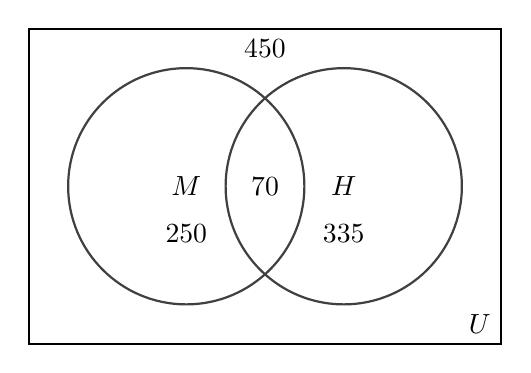
\begin{tikzpicture}[scale=1.0]
	\def\circleA{(0,0) circle (1.5)} %A
	\def\circleB{(0:2) circle (1.5)} %B

	\colorlet{circle edgeA}{black!75} 
	\colorlet{circle areaA}{red!100}
	\colorlet{circle edgeB}{black!75} 
	\colorlet{circle areaB}{green!100}

	\tikzset{
		filledA/.style={fill=circle areaA, draw=circle edgeA, thick},
		filledB/.style={fill=circle areaB, draw=circle edgeB, thick},
		outlineA/.style={draw=circle edgeA, thick},
		outlineB/.style={draw=circle edgeB, thick},
	}

	\begin{scope}[fill opacity=0.5]         
			%\fill[filledB] \circleB;    
			%\fill[filledA] \circleA;
	\end{scope}

	\draw[outlineA] \circleA node {$M$} node[below=10pt] {$250$}; 
	\draw[outlineB] \circleB node {$H$} node[below=10pt] {$335$}; 
	\node at (0:1) {$70$}; %%intersection node%%
	\node[anchor=south] at (current bounding box.north) {$450$}; 
	\draw[thick] (-2,-2) rectangle (4,2) node[anchor=south east] at (current bounding box.south east) {$U$}; 
\end{tikzpicture} 
\end{enumerate}
\item [(b)]$n(H\cap H)=70$
\item [(c)]$n(H-M)=335$
\item [(d)]$n(M\cup H)=250+70+335=655$
\item [(e)]$n\left((M\cup H)'\right)=n(U)-n(M\cup H)=1105-655=450$\vfill
\end{enumerate}
\end{enumerate}
\item \emph{Survivor}, \emph{CSI}, and \emph{ER} all belong to the Thursday
night prime time lineup. A group of $600$ college students were surveyed.
$350$ students watch \emph{Survivor}, $280$ watch \emph{CSI}, and
$320$ watch \emph{ER}. $50$ students watch all three shows. $190$
students watch both \emph{Survivor} and \emph{ER}. $180$ students
watch both \emph{Survivor} and \emph{CSI}. $50$ students watch only
\emph{ER}.

\begin{enumerate}
\item Construct a Venn diagram, and write the appropriate numbers in the
eight regions.
\item How many students watch only \emph{Survivor}?
\item How many students watch \emph{CSI }or \emph{Survivor}?
\item How many students watch \emph{CSI }or \emph{ER}?
\item How many students watch only \emph{CSI}?

\begin{enumerate}
\item [(a)]Number in $S$ and $ER$ but not $CSI$ is: $190-50=140$, Number
in $S$ and $CSI$ but not $ER$ is: $180-50=130$. Number in $CSI$
and $ER$ but not $S$ is: $320-50-140-50=80$. Number only in $S$
is: $350-130-50-140=30$. Number only in $CSI$ is: $280-130-50-80=20$.

\begin{enumerate}
\item []\def\firstcircle{(90:1.75cm) circle (2.5cm)} 
\def\secondcircle{(210:1.75cm) circle (2.5cm)} 
\def\thirdcircle{(330:1.75cm) circle (2.5cm)}

\begin{tikzpicture}[scale=.6]    
\begin{scope}     
	\fill[white]\firstcircle;       
	\fill[white] \secondcircle;       
	\fill[white] \thirdcircle;     
\end{scope}     
\begin{scope}
	\clip 
	\secondcircle;       
	\fill[white] 
	\firstcircle;     
\end{scope}     
\begin{scope}       
	\clip 
	\secondcircle;       
	\fill[white] 
	\thirdcircle;     
\end{scope}     
\begin{scope}       
	\clip 
	\firstcircle;       
	\fill[white] 
	\thirdcircle;     
\end{scope}     
\begin{scope}       
	\clip \firstcircle;       
	\clip \secondcircle;       
	\fill[white] \thirdcircle;     
\end{scope}     
\draw 
	\firstcircle node[text=black] {$S$} node[above=10pt] {$30$};     
\draw 
	\secondcircle node [text=black,below left] {$CSI$} node[below left=10pt] {$20$};     
\draw 
	\thirdcircle node [text=black,below right] {$ER$} node[below right=10pt] {$50$};     
\begin{scope}[font=\small]       
	\node(0,0) {$50$}; %AnBnC       
	\draw(30:1.5cm) node {$140$}; %AnC       
	\draw(150:1.5cm) node {$130$}; %AnB       
	\draw(270:1.5cm) node {$80$}; %BnC    
\end{scope}

\draw[thick] (-4.8,-3.55) rectangle (4.75,4.4) node[anchor=south east] at (current bounding box.south east) {$U$} node[anchor=north west] at (current bounding box.north west) {$100$}; 

\end{tikzpicture}
\end{enumerate}
\item [(b)]From diagram:$30$
\item [(c)]From diagram: $30+130+140+50+80+20=450$, or by the union rule:
$350+280-180=450$.
\item [(d)]From diagram: $20+130+50+80+140+50=570$, or by the union rule:
$280+320-130=470$
\item [(e)]From diagram: $20$
\end{enumerate}
\end{enumerate}
\end{enumerate}
\vfill
\begin{enumerate}[resume]
\item Find the value of each of the following:

\begin{enumerate}
\item $4!$

\begin{enumerate}
\item []$4!=4\cdot3\cdot2\cdot1=24$
\end{enumerate}
\item $7!$

\begin{enumerate}
\item []$7!=7\cdot6\cdot5\cdot4\cdot3\cdot2\cdot1=5040$
\end{enumerate}
\item $0!$

\begin{enumerate}
\item []$0!=1$
\end{enumerate}
\item $\frac{10!}{7!}$

\begin{enumerate}
\item []$\frac{10!}{7!}=\frac{10\cdot9\cdot8\cdot\cancel{7}\cdot\cancel{6}\cdot\cancel{5}\cdot\cancel{4}\cdot\cancel{3}\cdot\cancel{2}\cdot\cancel{1}}{\cancel{7}\cdot\cancel{6}\cdot\cancel{5}\cdot\cancel{4}\cdot\cancel{3}\cdot\cancel{2}\cdot\cancel{1}}=720$
\end{enumerate}
\item $\frac{27!}{4!25!}$

\begin{enumerate}
\item []$\frac{27!}{4!25!}=\frac{27\cdot26}{4!\cdot1}=\frac{702}{24}=117$.
Similarly to above, everything before $25$ cancels out. 
\end{enumerate}
\item $\frac{1000!}{998!}$

\begin{enumerate}
\item []$\frac{1000!}{998!}=\frac{1000\cdot999}{1}=999,000$. Similarly
to above, everything before $999$ cancels out. 
\end{enumerate}
\item $_{7}P_{2}$

\begin{enumerate}
\item []$_{7}P_{2}=\frac{7!}{(7-2)!}=\frac{7!}{5!}=\frac{5040}{120}=42$
or $\frac{7!}{5!}=7\cdot6=42$.
\end{enumerate}
\item $_{6}C_{4}$

\begin{enumerate}
\item []$_{6}C_{4}=\frac{6!}{(6-4)!4!}=\frac{6!}{2!4!}=\frac{6\cdot5}{2!}=\frac{30}{2}=15$
\end{enumerate}
\end{enumerate}
\end{enumerate}
\vfill
\begin{enumerate}[resume]
\item A certain model of pickup truck is available in five exterior colors,
three interior colors, and three interior styles. In addition, the
transmission can be either manual or automatic, and the truck can
have either two-wheel or four-wheel drive. How many different versions
of the pickup truck can be ordered?

\begin{enumerate}[resume]
\item []We have five categories, $\underline{\,\,\,\,\,}\times\underline{\,\,\,\,\,}\times\underline{\,\,\,\,\,}\times\underline{\,\,\,\,\,}\times\underline{\,\,\,\,\,}$.
Filling in the number of choices for each category we have, 
\[
\underline{5}\times\underline{3}\times\underline{3}\times\underline{2}\times\underline{2}=180
\]
\end{enumerate}
\end{enumerate}
\vfill
\begin{enumerate}[resume]
\item A certain fraternity must elect a president, vice president, and treasurer
from its 30 members. How many ways can this be done?

\begin{enumerate}[resume]
\item []There are no repeats and order does matter (since order will determine
who is pres., vice pres., and treasurer). So we use permutations,
\begin{eqnarray*}
_{30}P_{3}=\frac{30!}{(30-3)!}=\frac{30!}{27!} & = & 30\cdot29\cdot28=24,360
\end{eqnarray*}
\end{enumerate}
\end{enumerate}
\vfill
\begin{enumerate}[resume]
\item The local branch of a national business chain has 27 employees. If
they all shake each other's hand at the company picnic, at least how
many handshakes occurred?

\begin{enumerate}
\item []There are no repeats and order does NOT matter (Joe shaking hands
with Betty is the same as Betty shaking hands with Joe). So we use
combinations,
\[
_{27}C_{2}=\frac{27!}{(27-2)!2!}=\frac{27!}{25!2!}=\frac{27\cdot26}{2}=351
\]
\end{enumerate}
\end{enumerate}
\vfill
\begin{enumerate}[resume]
\item Using a standard deck of $52$ cards, 

\begin{enumerate}
\item how many ways can five cards be drawn?
\item how many five card hands can be dealt?

\begin{enumerate}
\item [(a)]Here order matters, e.g., $\{7\heartsuit,K\spadesuit,2\spadesuit,3\clubsuit,3\diamondsuit\}$
is a different way to draw the cards then $\{2\spadesuit,3\clubsuit,3\diamondsuit,7\heartsuit,K\spadesuit,\}$
since the order is different. So we use permutations,
\[
_{52}P_{5}=\frac{52!}{(52-5)!}=\frac{52!}{47!}=311,875,200
\]
\item [(b)]Here order does not matter, e.g., $\{7\heartsuit,K\spadesuit,2\spadesuit,3\clubsuit,3\diamondsuit\}$
is the same hand as $\{2\spadesuit,3\clubsuit,3\diamondsuit,7\heartsuit,K\spadesuit,\}$.
So we use combinations, 
\[
_{52}C_{5}=\frac{52!}{(52-5)!5!}=2,598,960
\]
\end{enumerate}
\end{enumerate}
\end{enumerate}
\vfill
\begin{enumerate}[resume]
\item A three-person committee must be chosen from a group of ten men and
twelve women. How many committees are possible if it must consist
of the following?

\begin{enumerate}
\item Three men.
\item Three women.
\item One woman and two men.
\item One man and two women.
\item One man and two women, and one of these is selected as a spokesperson
of the committee.

\begin{enumerate}
\item [(a)]No repeats and order doesn't matter$\Rightarrow$combination.
$_{10}C_{3}=\frac{10!}{(10-3)!3!}=\frac{10\cdot9\cdot8}{3!}=\frac{720}{6}=120$
\item [(b)]No repeats and order doesn't matter$\Rightarrow$combination.
$_{12}C_{3}=\frac{12!}{(12-3)!3!}=\frac{12\cdot11\cdot10}{3!}=\frac{1320}{6}=220$
\item [(c)]Here we have two categories: $\underline{\,\,\,\,\,}\times\underline{\,\,\,\,\,}$.
For the first categories we have $12$ choices (equivalently, $_{12}C_{1}=\frac{12!}{(12-1)!1!}=12$),
and for the second we have $_{10}C_{2}=\frac{10!}{(10-2)!2!}=\frac{10\cdot9}{2}=45$.
\\
So we have $12\times45=540$ posibilities.
\item [(d)]Similarly to above, we have two categories. For the first categories
we have $10$ choices, and for the second we have $_{12}C_{2}=\frac{12!}{(12-2)!2!}=\frac{12\cdot11}{2}=66$.
Then we select one of the three to be a spokesperson. \\
So we have $10\times66\times3=1980$ posibilities.
\item []Equivalently, use a permutation where the order of $2$ members
does not matter, $\nicefrac{\left(10\times\frac{12!}{10!}\times3\right)}{2!}=1980$
(like counting the ways to arrange the letters in ``SCHOOL''; the
order of the ``O'''s does not mater).
\end{enumerate}
\end{enumerate}
\end{enumerate}
\vfill
\begin{enumerate}[resume]
\item Each student at State University has a student ID number consisting
of five digits (the first digit is nonzero, and the digits can be
repeated) followed by two of the letters $A$, $B$, $C$, and $D$
(letters cannot be repeated). How many different student numbers are
possible?

\begin{enumerate}
\item []We have five numbers $0-9$ which can be repeated, but the the
first is nonzero: $9\times10\times10\times10\times10=9\cdot10^{4}=90,000$
possibilities, and then two of four letters which cannot be repeated.
It is implied that the order of the letters does matter since $10000AB$
and $10000BA$ would be two different IDs. So for the letters we have,
$_{4}P_{2}=\frac{4!}{(4-2)!}=\frac{24}{2}=12$ possibilities. For
a total of $9\times10^{4}\times12=1,080,000$ possible ID numbers.\vfill
\end{enumerate}
\end{enumerate}

\end{document}
